\documentclass[letterpaper,10pt]{article}

\usepackage{enumitem}
\usepackage{titling}
\usepackage{listings,listings-rust}
\usepackage{url}
\usepackage{soul}
\usepackage{hyperref}
\usepackage{setspace}
\usepackage{subfig}
\usepackage{sectsty}
\usepackage{pdfpages}
\usepackage{colortbl}
\usepackage{multirow}
\usepackage{multicol}
\usepackage{relsize}
\usepackage{amsmath}
\usepackage{wasysym}
\usepackage{fancyvrb}
\usepackage[yyyymmdd]{datetime}
\usepackage{amsmath,amssymb,amsthm,graphicx,xspace}
\usepackage[titlenotnumbered,noend,noline]{algorithm2e}
\usepackage[compact]{titlesec}
\usepackage{XCharter}
\usepackage[T1]{fontenc}
\usepackage[scaled]{beramono}
\usepackage[normalem]{ulem}
\usepackage{booktabs}
\usepackage{tikz}
\usetikzlibrary{arrows.meta,automata,shapes,trees,matrix,chains,scopes,positioning,calc,decorations.pathreplacing}
\tikzstyle{block} = [rectangle, draw, fill=blue!20, 
    text width=2.5em, text centered, rounded corners, minimum height=2em]
\tikzstyle{bw} = [rectangle, draw, fill=blue!20, 
    text width=4em, text centered, rounded corners, minimum height=2em]

\definecolor{namerow}{cmyk}{.40,.40,.40,.40}
\definecolor{namecol}{cmyk}{.40,.40,.40,.40}
\renewcommand{\dateseparator}{-}

\let\LaTeXtitle\title
\renewcommand{\title}[1]{\LaTeXtitle{\textsf{#1}}}

\lstset{basicstyle=\footnotesize\ttfamily,breaklines=true}

\newcommand{\CPP}{C\nolinebreak\hspace{-.05em}\raisebox{.4ex}{\tiny\bf +}\nolinebreak\hspace{-.10em}\raisebox{.4ex}{\tiny\bf +}}
\def\CPP{{C\nolinebreak[4]\hspace{-.05em}\raisebox{.4ex}{\tiny\bf ++}}}

\newcommand{\handout}[5]{
  \noindent
  \begin{center}
  \framebox{
    \vbox{
      \hbox to 5.78in { {\bf ECE459: Programming for Performance } \hfill #2 }
      \vspace{4mm}
      \hbox to 5.78in { {\Large \hfill #4  \hfill} }
      \vspace{2mm}
      \hbox to 5.78in { {\em #3 \hfill \today} }
    }
  }
  \end{center}
  \vspace*{4mm}
}

\newcommand{\lecture}[3]{\handout{#1}{#2}{#3}{Lecture#1}}
\newcommand{\tuple}[1]{\ensuremath{\left\langle #1 \right\rangle}\xspace}

\addtolength{\oddsidemargin}{-1.000in}
\addtolength{\evensidemargin}{-0.500in}
\addtolength{\textwidth}{2.0in}
\addtolength{\topmargin}{-1.000in}
\addtolength{\textheight}{1.75in}
\addtolength{\parskip}{\baselineskip}
\setlength{\parindent}{0in}
\renewcommand{\baselinestretch}{1.5}
\newcommand{\term}{Winter 2020}

\singlespace


\begin{document}

\lecture{25 --- Profiling}{\term}{Jeff Zarnett \& Patrick Lam}

\section*{Profiling}

Think back to the beginning of the course when we did a quiz on what operations are fast and what operations are not. The important takeaway was not that we needed to focus on how to micro-optimize this abstraction or that hash function, but that our intuition about what is fast and what is slow is often wrong. Not just at a macro level, but at a micro level. You may be able to narrow down that this computation of $x$ is slow, but if you examine it carefully\ldots what parts of it are slow?

If you don't use tools, then you end up guessing. You just make some assumptions about what you think is likely to be slow and try to change it. You've probably heard the famous quotation before, but here it is in its full form:

\begin{quote}
\textit{Programmers waste enormous amounts of time thinking about, or worrying about, the speed of noncritical parts of their programs, and these attempts at efficiency actually have a strong negative impact when debugging and maintenance are considered. We should forget about small efficiencies, say about 97\% of the time: premature optimization is the root of all evil. Yet we should not pass up our opportunities in that critical 3\%.}
\end{quote}
	\hfill -- Donald Knuth

So going about this blindly is probably a waste of time. You might be fortunate and optimize a slow part\footnote{There is a saying that even a blind squirrel sometimes finds a nut.} but we should really follow one of my favourite rules: ``don't guess, measure!''\footnote{Now I am certain you are sick of hearing that.} So, to make your programs or systems fast, you need to find out what is currently slow and improve it (duh!). Up until now in the course it's mostly been about ``let's speed this up'', but we did not take much time to decide what we should speed up (though you maybe did this on an assignment\ldots?).

The general idea is, collect some data on what parts of the code are taking up the majority of the time. This can be broken down into looking at what functions get called, or how long functions take, or what's using memory\ldots

There is always the ``informal'' or ``ad-hoc'' way of doing this; it works but it's often not the best plan. You probably know that when developing a program you can ``debug'' it without using any tools (e.g., \texttt{gdb}) by inserting print statements to the console or the log file. So when you enter function \texttt{foo} you print a nice little line on the console that say something like ``entering function foo'', associated with a timestamp and then when you're ready to return, a corresponding print function that says ``exiting'' appears, also with a timestamp.

I've used this approach myself to figure out what blocks of a single large function are taking a long time (such as a time when I found out that updating exchange rates was slow.). But this approach is not necessarily a good one.  It's an example of ``invasive'' profiling---we are going in and changing the source code of the program in question---to add (slow!) instrumentation (log/debug statements). Plus we have to do a lot of manual accounting. Assuming your program is fast and goes through functions quickly and often, trying to put the pieces together manually is hopeless. It worked in that one example because the single function itself was running in the half-hour range and I could see that the save operation was taking twelve minutes. Not kidding.

I also mentioned earlier that I used the profiling tool for CUDA to find out what was wrong with my N-Body program. I ran the command \texttt{nvprof target/release/nbody-cuda}, and in addition to the regular program output I got the following, which showed that the time was going to the kernel and I wasn't losing a lot in overhead:

{\scriptsize
\begin{verbatim}
==20734== Profiling application: target/release/nbody-cuda
==20734== Profiling result:
            Type  Time(%)      Time     Calls       Avg       Min       Max  Name
 GPU activities:  100.00%  10.7599s         1  10.7599s  10.7599s  10.7599s  calculate_forces
                    0.00%  234.72us         2  117.36us  100.80us  133.92us  [CUDA memcpy HtoD]
                    0.00%  94.241us         1  94.241us  94.241us  94.241us  [CUDA memcpy DtoH]
      API calls:   97.48%  10.7599s         1  10.7599s  10.7599s  10.7599s  cuStreamSynchronize
                    1.92%  211.87ms         1  211.87ms  211.87ms  211.87ms  cuCtxCreate
                    0.54%  59.648ms         1  59.648ms  59.648ms  59.648ms  cuCtxDestroy
                    0.04%  4.8704ms         1  4.8704ms  4.8704ms  4.8704ms  cuModuleLoadData
                    0.00%  404.72us         2  202.36us  194.51us  210.21us  cuMemAlloc
                    0.00%  400.58us         2  200.29us  158.08us  242.50us  cuMemcpyHtoD
                    0.00%  299.30us         2  149.65us  121.42us  177.88us  cuMemFree
                    0.00%  243.86us         1  243.86us  243.86us  243.86us  cuMemcpyDtoH
                    0.00%  85.000us         1  85.000us  85.000us  85.000us  cuModuleUnload
                    0.00%  41.356us         1  41.356us  41.356us  41.356us  cuLaunchKernel
                    0.00%  18.483us         1  18.483us  18.483us  18.483us  cuStreamCreateWithPriority
                    0.00%  9.0780us         1  9.0780us  9.0780us  9.0780us  cuStreamDestroy
                    0.00%  2.2080us         2  1.1040us     215ns  1.9930us  cuDeviceGetCount
                    0.00%  1.4600us         1  1.4600us  1.4600us  1.4600us  cuModuleGetFunction
                    0.00%  1.1810us         2     590ns     214ns     967ns  cuDeviceGet
                    0.00%     929ns         3     309ns     230ns     469ns  cuDeviceGetAttribute
\end{verbatim}
}

Oh, and for comparison, here's the one where I make much better use of the GPU's capabilities (with better grid and block settings):

{\scriptsize
\begin{verbatim}
=22619== Profiling result:
            Type  Time(%)      Time     Calls       Avg       Min       Max  Name
 GPU activities:   99.92%  417.53ms         1  417.53ms  417.53ms  417.53ms  calculate_forces
                    0.06%  236.03us         2  118.02us  101.44us  134.59us  [CUDA memcpy HtoD]
                    0.02%  93.057us         1  93.057us  93.057us  93.057us  [CUDA memcpy DtoH]
      API calls:   52.09%  417.54ms         1  417.54ms  417.54ms  417.54ms  cuStreamSynchronize
                   26.70%  214.00ms         1  214.00ms  214.00ms  214.00ms  cuCtxCreate
                   13.63%  109.26ms         1  109.26ms  109.26ms  109.26ms  cuModuleLoadData
                    7.42%  59.502ms         1  59.502ms  59.502ms  59.502ms  cuCtxDestroy
                    0.05%  364.08us         2  182.04us  147.65us  216.42us  cuMemcpyHtoD
                    0.04%  306.48us         2  153.24us  134.10us  172.37us  cuMemAlloc
                    0.04%  285.73us         2  142.86us  122.90us  162.83us  cuMemFree
                    0.03%  246.37us         1  246.37us  246.37us  246.37us  cuMemcpyDtoH
                    0.01%  61.916us         1  61.916us  61.916us  61.916us  cuModuleUnload
                    0.00%  26.218us         1  26.218us  26.218us  26.218us  cuLaunchKernel
                    0.00%  15.902us         1  15.902us  15.902us  15.902us  cuStreamCreateWithPriority
                    0.00%  9.0760us         1  9.0760us  9.0760us  9.0760us  cuStreamDestroy
                    0.00%  1.6720us         2     836ns     203ns  1.4690us  cuDeviceGetCount
                    0.00%  1.0950us         1  1.0950us  1.0950us  1.0950us  cuModuleGetFunction
                    0.00%     888ns         3     296ns     222ns     442ns  cuDeviceGetAttribute
                    0.00%     712ns         2     356ns     212ns     500ns  cuDeviceGet
\end{verbatim}
}


Nicholas Nethercote wrote the ``counts'' tool\footnote{\url{https://github.com/nnethercote/counts}} to process ad-hoc debug output and shows an example of using it to profile the size of heap allocations in Firefox. In the example in the README, he reports that while most allocations are small, most memory is allocated as part of a large allocation. He provides a number of other examples where ad-hoc profiling is useful: how often are certain paths executed? how many times does a loop iterate? how many elements are in a hash table at a given location? And more! It's hard to write a general-purpose tool for these ad-hoc queries.

(Also like debugging, if you get to be a wizard you can maybe do it by code inspection, but that technique of speculative execution inside your head is a lot harder to apply to performance problems than it is to debugging. Trained professionals like Nicholas Nethercote use profilers, so you can too.)

So we should all agree, we want to use tools and do this in a methodical way.

Now that we agree on that, let's think about how profiling tools work\:

\begin{itemize}[noitemsep]
\item sampling-based (traditional): every so often (e.g. 100ms for gprof), stop the system and ask it what it's doing (query the system state); or,
\item instrumentation-based, or probe-based/predicate-based
  (sometimes, too expensive): query system state under certain
  conditions; like conditional breakpoints.
\end{itemize}
We'll talk about both per-process profiling and system-wide profiling. You can read more about profiling in Chapter 5 (Profiling) of The Rust Performance Book~\cite{nethercote20:_rust_perfor_book}; it discusses heap profiling in much more detail than we do (or don't,
more accurately).

If you need your system to run fast, you need to start profiling
and benchmarking as soon as you can run the system. Benefits:
\begin{itemize}[noitemsep]
\item establishes a baseline performance for the system;
\item allows you to measure impacts of changes and further system development;
\item allows you to re-design the system before it's too late;
\item avoids the need for ``perf spray'' to make the system faster, since
that spray is often made of ``unobtainium''\footnote{\url{http://en.wikipedia.org/wiki/Unobtainium}}.
\end{itemize}

\paragraph{Tips for Leveraging Profiling.}
When writing large software projects:
  \begin{itemize}[noitemsep]
    \item First, write clear and concise code. Don't do any premature optimizations---focus on correctness. Still, there are choices you can make that support performance at this stage, like using an efficient search or sort algorithm, if you know it's better and won't take additional effort.
    \item Once it's working, profile to get a baseline of your performance: it allows you to easily track any performance changes and to re-design your program before it's too late.
  \end{itemize}
Focus your optimization efforts on the code that matters.

Look for abnormalities; in particular, you're looking for
deviations from the following rules:
\begin{itemize}[noitemsep]
\item time is spent in the right part of the system/program;
\item time is not spent in error-handling, noncritical code, or exceptional cases; and
\item time is not unnecessarily spent in the operating system.
\end{itemize}
For instance, ``why is {\tt ps} taking up all my cycles?'';
see page 34 of ~\cite{300ps}.

\paragraph{Development vs. production.}
You can always profile your systems in development, but that might not
help with complexities in production. (You want separate dev and
production systems, of course!) We'll talk a bit about DTrace, which
is one way of profiling a production system. The constraints on profiling 
production systems are that the profiling must not affect the system's
performance or reliability.

\section*{Userspace per-process profiling}
Sometimes---or, in this course, often---you can get away with
investigating just one process and get useful results about that
process's behaviour.  We'll first talk about {\tt perf}, the profiler 
recommended for use with Rust. This is Linux-specific, though.

The \texttt{perf} tool is an interface to the Linux kernel's built-in
sample-based profiling using CPU counters. It works per-process, per-CPU, or system-wide. It can report the cost of each line of code.

Webpage: \url{https://perf.wiki.kernel.org/index.php/Tutorial}

\noindent
Here's a usage example on some old assignment code from a previous offering of the course:
\begin{lstlisting}[basicstyle=\scriptsize]
[plam@lynch nm-morph]$ perf stat ./test_harness

 Performance counter stats for './test_harness':

       6562.501429 task-clock                #    0.997 CPUs utilized          
               666 context-switches          #    0.101 K/sec                  
                 0 cpu-migrations            #    0.000 K/sec                  
             3,791 page-faults               #    0.578 K/sec                  
    24,874,267,078 cycles                    #    3.790 GHz                     [83.32%]
    12,565,457,337 stalled-cycles-frontend   #   50.52% frontend cycles idle    [83.31%]
     5,874,853,028 stalled-cycles-backend    #   23.62% backend  cycles idle    [66.63%]
    33,787,408,650 instructions              #    1.36  insns per cycle        
                                             #    0.37  stalled cycles per insn [83.32%]
     5,271,501,213 branches                  #  803.276 M/sec                   [83.38%]
       155,568,356 branch-misses             #    2.95% of all branches         [83.36%]

       6.580225847 seconds time elapsed
\end{lstlisting} %$

Right, let's get started. We're going to use the blog post~\cite{rustflamegraph} as a guide; that source tells a more complete story of an example of using the profiler to optimize, but for now we are just interested in the steps.

The first thing to do is to compile with debugging info, go to your \texttt{Cargo.toml} file and add:
\begin{verbatim}
[profile.release]
debug = true
\end{verbatim}

This means that \texttt{cargo build --release} will now compile the version with debug info (you can tell because it will say \texttt{Finished release [optimized + debuginfo] target(s) in 0.55s}; without this, we wouldn't get the part that says debug info so we can tell if it's correct. And we want it to be the release version that we're instrumenting, because we want the compiler optimizations to be applied. Without those, we might be trying to optimize things where the compiler would do it for us anyway.

The basic plan is to run the program using \texttt{perf record}, which will sample the execution of the program to produce a data set. Then there are three ways we can look at the code: \texttt{perf report}, \texttt{perf annotate}, and a flamegraph. We'll look at all of those, but in a live demo.


\paragraph{CLion.} While we've seen how to use \texttt{perf}, it's not the only way. During development of some of the code exercises, I used the CLion built-in profiler for this purpose. It generates a flamegraph for you too, and I'll show that for how to create the flamegraph as well.

\section*{Profiler Guided Optimization (POGO)}

In 2015 we were fortunate enough to have a guest lecture from someone at Microsoft actually in the room to give the guest lecture on the subject of Profile Guided Optimization (or POGO). In subsequent years, I was not able to convince him to fly in just for the lecture. Now there's a pandemic, so that's a big nope. Anyway, let's talk about the subject, which is by no means restricted to Rust.

The compiler does static analysis of the code you've written and makes its best guesses about what is likely to happen. The canonical example for this is branch prediction: there is an if-else block and the compiler will then guess about which is more likely and optimize for that version. Consider three examples, originally from~\cite{pogo} but replaced with some Rust equivalents:

\begin{lstlisting}[language=Rust]
fn which_branch(a: i32, b: i32) {
    if a < b {
        println!("Case one.");
    } else {
        println!("Case two.");
    }
}
\end{lstlisting}

Just looking at this, which is more likely, \texttt{a < b} or \texttt{a >= b}? Assuming there's no other information in the system the compiler can believe that one is more likely than the other, or having no real information, use a fallback rule. This works, but what if we are wrong? Suppose the compiler decides it is likely that \texttt{a} is the larger value and it optimizes for that version. However, it is only the case 5\% of the time, so most of the time the prediction is wrong. That's unpleasant. But the only way to know is to actually run the program.

\begin{multicols}{2}
\begin{lstlisting}[language=Rust]
trait Polite {
    fn greet(&self) -> String;
}

struct Kenobi {
    /* Stuff */
}
impl Polite for Kenobi {
    fn greet(&self) -> String {
        return String::from("Hello there!");
    }
}
\end{lstlisting}
\columnbreak
\begin{lstlisting}[language=Rust]
struct Grievous {
    /* Things */
}
impl Polite for Grievous {
    fn greet(&self) -> String {
        return String::from("General Kenobi.");
    }
}

fn devirtualization(thing: &Polite) {
    println!("{}", thing.greet());
}

\end{lstlisting}
\end{multicols}



There are similar questions raised for the other two examples. What is the ``normal'' type for some reference \texttt{thing}? It could be of either type \texttt{Kenobi} or \texttt{Grievous}. If we do not know, the compiler cannot do devirtualization (replace this virtual call with a real one). If there was exactly one type that implements the \texttt{Polite} trait we wouldn't have to guess. But are we much more likely to see \texttt{Kenobi} than \texttt{Grievous}?

\begin{lstlisting}[language=Rust]
fn match_thing(x: i32) -> i32 {
    match x {
        0..10 => 1,
        11..100 => 2,
        _ => 0
    }
}
\end{lstlisting}

 Same thing with \texttt{x}: what is its typical value? If we know that, it is our prediction. Actually, in a match block with many options, could we rank them in descending order of likelihood?

There exists a solution to this, and it is that we can give hints to the compiler, but that's a manual process. Automation is a good thing and this lecture is about that. These sorts of things already exist for Java! The Java HotSpot virtual machine will update its predictions on the fly. There are some initial predictions and if they turn out to be wrong, the Just In Time compiler will replace it with the other version. That's neat! I don't know for certain but I suspect the .NET runtime will do the same for something like C\#. But this is Rust and we don't have the runtime to reduce the overhead: the compiler runs and it does its job and that's it; the program is never updated with newer predictions if more data becomes known.

Solving this problem is the goal of POGO. It is taking the data from some actual runs of the program and using that to inform the predictions. This necessitates a multi-step compile: first compile the code, run it to collect data, then recompile the code using the data we collected. Let's expand on all three steps.

Step one is to generate an executable with instrumentation. Ask to compile with instrumentation enabled, which also says what directory to put it in: \texttt{-Cprofile-generate=/tmp/pgo-data}. The compiler inserts a bunch of probes into the generated code that are used to record data. Three types of probe are inserted: function entry probes, edge probes, and value probes.  A function entry probe, obviously, counts how many times a particular function is called. An edge probe is used to count the transitions (which tells us whether an if branch is taken or the else condition). Value probes are interesting; they are used to collect a histogram of values. Thus, we can have a small table that tells us the frequency of what is given in to a \texttt{match} statement. When this phase is complete, there is an instrumented executable and an empty database file where the training data goes~\cite{pogo}. 

Step two is training day: run the instrumented executable through real-world scenarios. Ideally you will spend the training time on the performance-critical sections. It does not have to be a single training run, of course, data can be collected from as many runs as desired. Keep in mind that the program will run a lot slower when there's the instrumentation present. 

Still, it is important to note that you are not trying to exercise every part of the program (this is not unit testing); instead it should be as close to real-world-usage as can be accomplished. In fact, trying to use every bell and whistle of the program is counterproductive; if the usage data does not match real world scenarios then  the compiler has been given the wrong information about what is important. Or you might end up teaching it that almost nothing is important... 

According to the docs about it\footnote{\url{https://doc.rust-lang.org/rustc/profile-guided-optimization.html}}, the output \texttt{.profraw} files require a little bit of processing before they're ready to go. When the program is running, the recording of data is done as quickly as possible with little regard for making it neat. Think of it like taking notes furiously during a lecture and then later revisiting them to organize them a bit. The tool for doing this is \texttt{llvm-profdata} and it will organize the data into a \texttt{.profdata} file. We can merge multiple runs as needed into a single file that will be used for input. 

Step three is a recompile. This time, in addition to the source files, the (merged) training data is fed into the compiler for a second compile, and this data is applied to (hypothetically) produce a better output executable than could be achieved by static analysis alone.


It is not necessary to do all three steps for every build. Old training data can be re-used until the code base has diverged significantly enough from the instrumented version. According to~\cite{pogo}, the recommended workflow is for one developer to perform these steps and check the training data into source control so that other developers can make use of it in their builds.

The Intel Developer Zone explains the process in a handy infographic\footnote{Source: \url{https://software.intel.com/en-us/node/522721}} :

\begin{center}
	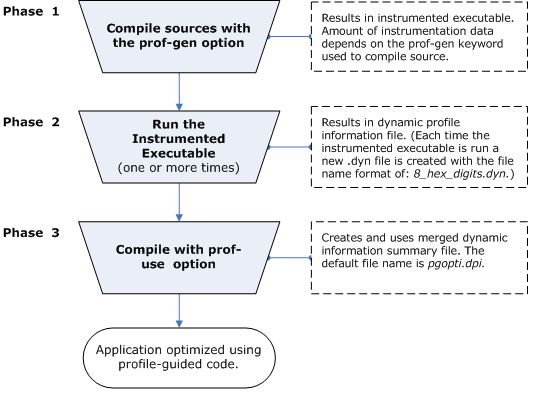
\includegraphics[width=0.5\textwidth]{images/pogo-workflow.jpg}
\end{center}



Or, here, a complete set of steps for actually running it if our program is all in \texttt{main.rs}, from the docs\footnote{\url{https://doc.rust-lang.org/rustc/profile-guided-optimization.html}}:

{\scriptsize
\begin{verbatim}
# STEP 1: Compile the binary with instrumentation
rustc -Cprofile-generate=/tmp/pgo-data -O ./main.rs

# STEP 2: Run the binary a few times, maybe with common sets of args.
#         Each run will create or update `.profraw` files in /tmp/pgo-data
./main mydata1.csv
./main mydata2.csv
./main mydata3.csv

# STEP 3: Merge and post-process all the `.profraw` files in /tmp/pgo-data
llvm-profdata merge -o ./merged.profdata /tmp/pgo-data

# STEP 4: Use the merged `.profdata` file during optimization. All `rustc`
#         flags have to be the same.
rustc -Cprofile-use=./merged.profdata -O ./main.rs
\end{verbatim}
}
(NB: Debian/Ubuntu's rustc doesn't seem to support PGO; I had to rustup it myself on my computer; I also used the Complete Cargo Workflow listed later.)

What does it mean for the executable to be better? We have already looked at an example about how to predict branches. Predicting it correctly will be faster than predicting it incorrectly, but this is not the only thing.  The algorithms will aim for speed in the areas that are ``hot'' (performance critical and/or common scenarios). The algorithms will alternatively aim to minimize the size of code of areas that are ``cold'' (not heavily used). It is recommended in~\cite{pogo} that less than 5\% of methods should be compiled for speed.

It is possible that we can combine multiple training runs and we can manually give some suggestions of what scenarios are important. Obviously the more a scenario runs in the training data, the more important it will be, as far as the POGO optimization routine is concerned, but multiple runs can be merged with user assigned weightings.

\subsection*{Behind the Scenes}

In the optimize phase, the training data is used to do the following optimizations( which I will point out are based on C and \CPP~ programs and not necessarily Rust, but the principles should work because the Rust compiler's approach to this is based on that of LLVM/Clang)~\cite{pogo2}:

\begin{multicols}{2}
\begin{enumerate}
\item Full and partial inlining
\item Function layout
\item Speed and size decision
\item Basic block layout 
\item Code separation
\item Virtual call speculation
\item Switch expansion
\item Data separation
\item Loop unrolling
\end{enumerate}
\end{multicols}

For the most part we should be familiar with the techniques that are listed as being other compiler optimizations we have previously discussed. The new ones are (3) speed and size decision, which we have just covered; and items (4) and (5) which relate to how to pack the generated code in the binary.

According to~\cite{pogo2} the majority of the performance gains relate to the inlining decisions. These decisions are based on the call graph path profiling: the behaviour of function \texttt{foo} may be very different when calling it from \texttt{bar} than it is when calling it from function \texttt{baz}. Let's look at this call graph from~\cite{pogo2}:

\begin{center}
	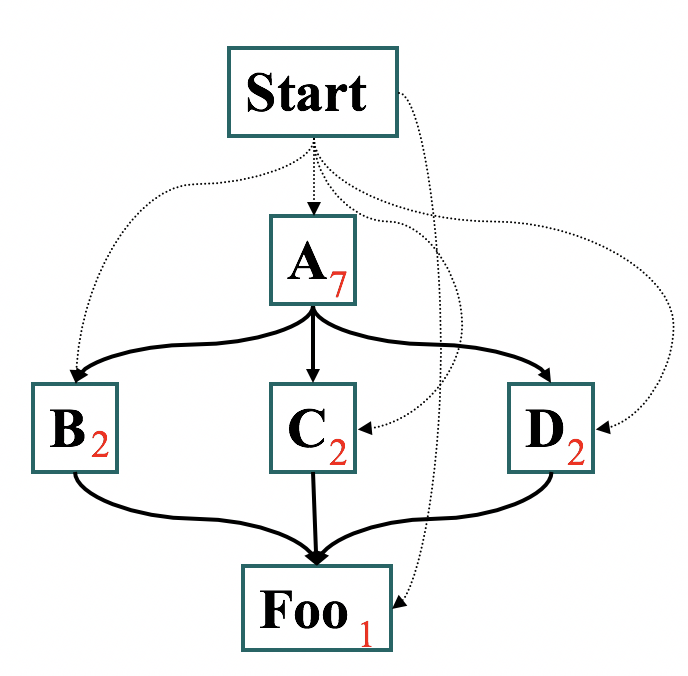
\includegraphics[width=0.25\textwidth]{images/callpaths.png}
\end{center}

Quick analysis of this code would have us find all the ways in which the functions might call each other. In total, there are 14 paths in this code, seven of which get us to function \texttt{Foo}. Consider another diagram showing the relationships between functions, in which the numbers on the edges represent the number of invocations~\cite{pogo2}:

\begin{center}
	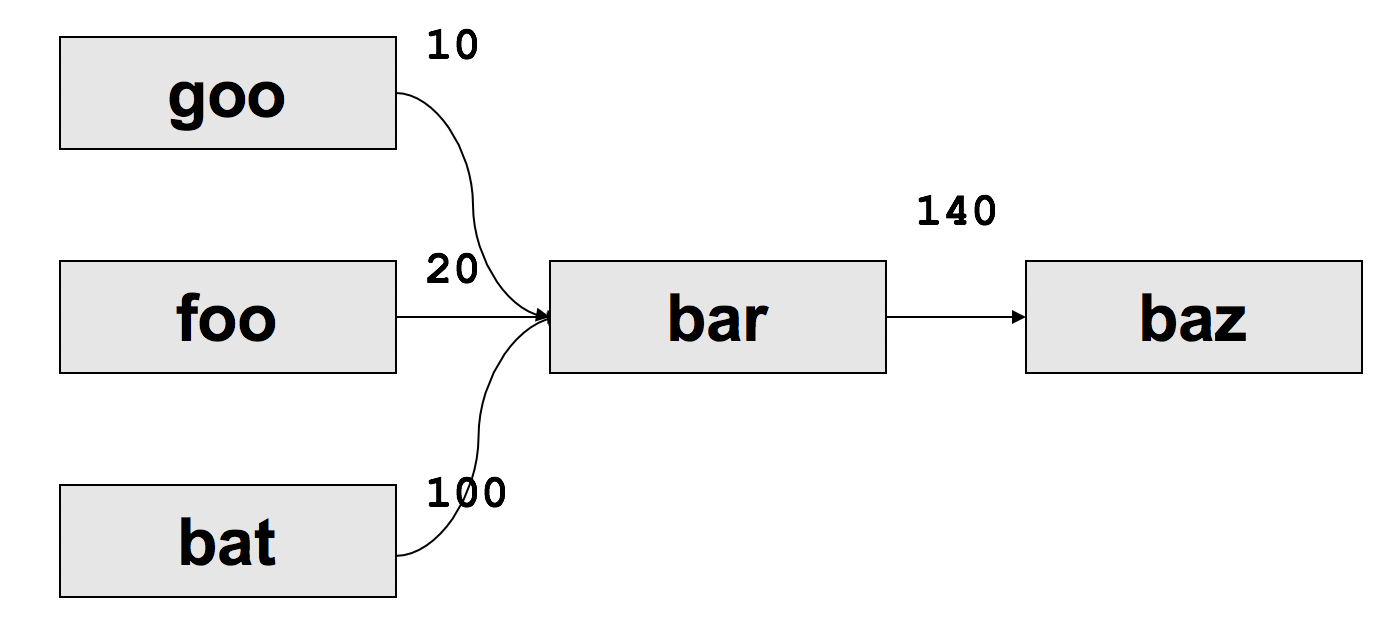
\includegraphics[width=0.4\textwidth]{images/callpaths2.png}
\end{center}

When considering what to do here, POGO takes the view like this~\cite{pogo2}:

\begin{center}
	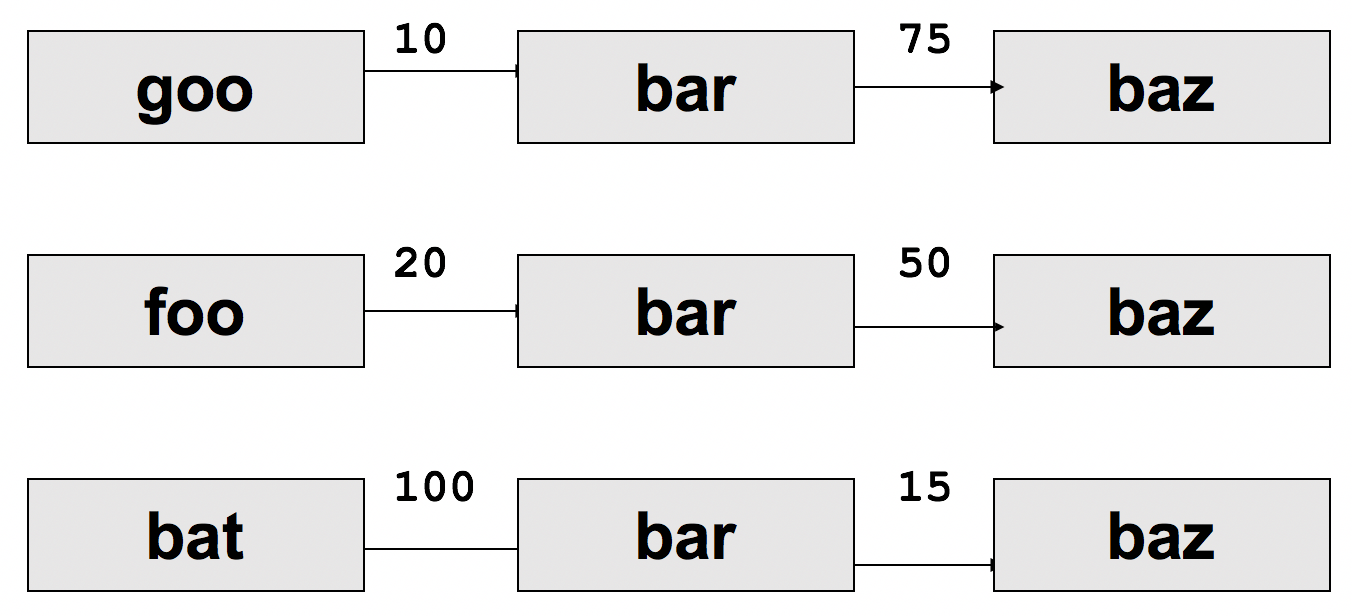
\includegraphics[width=0.4\textwidth]{images/callpaths3.png}
\end{center}

Each part of the call path is considered separately, remembering that we want to inline where it makes sense for speed, but otherwise leave it alone because of code size increases. Inlining \texttt{bar} into \texttt{bat} makes sense, but not inlining \texttt{bar} into \texttt{goo} (because that increases the code size without significant performance benefits). It also makes sense for \texttt{baz} to get inlined into \texttt{bar}. This is illustrated below~\cite{pogo2}:

\begin{center}
	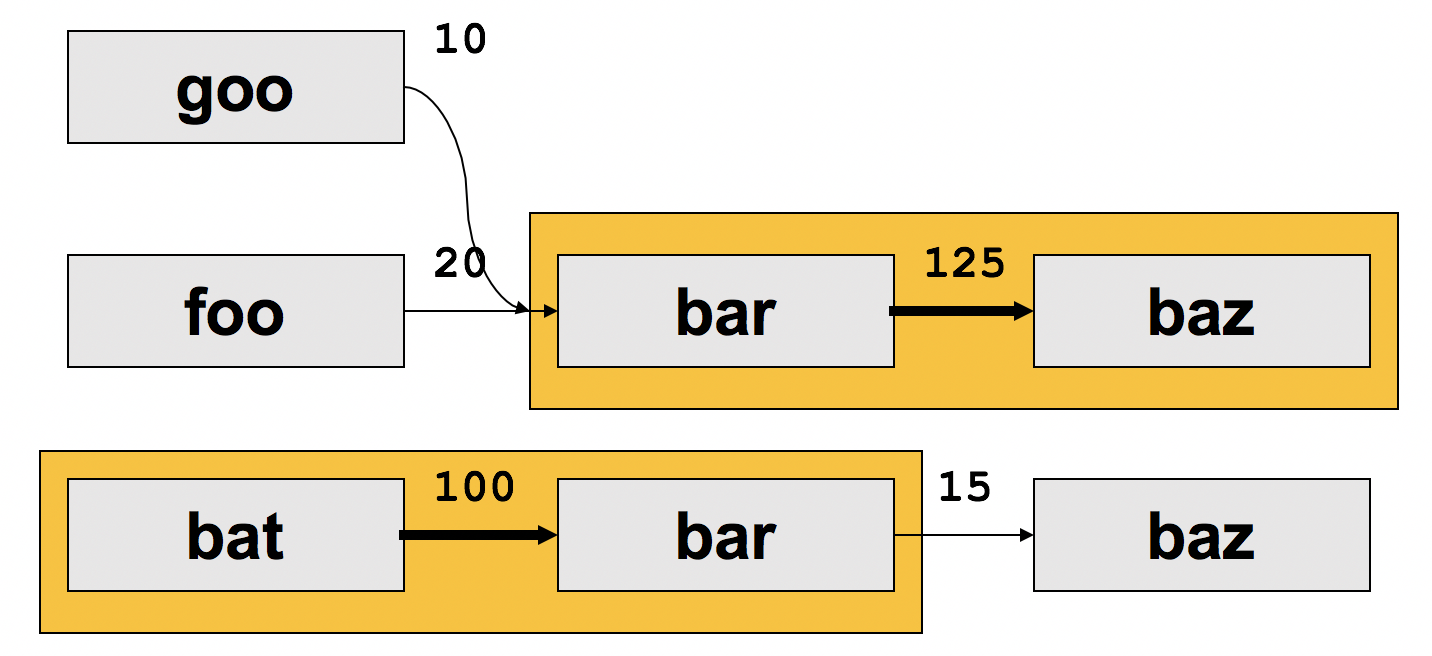
\includegraphics[width=0.4\textwidth]{images/callpaths4.png}
\end{center}

Packing the blocks is also done based on this call graph profiling. The most common cases will be put next to each other, and, where possible, subsequent steps are put next to each other. The more we can pack related code together, the fewer page faults we get by jumping to some other section, causing a cache miss... If the function being called is in the same page as the call, it has achieved ``page locality'' (and that is the goal!). This is represented visually~\cite{pogo2}:

\begin{center}
	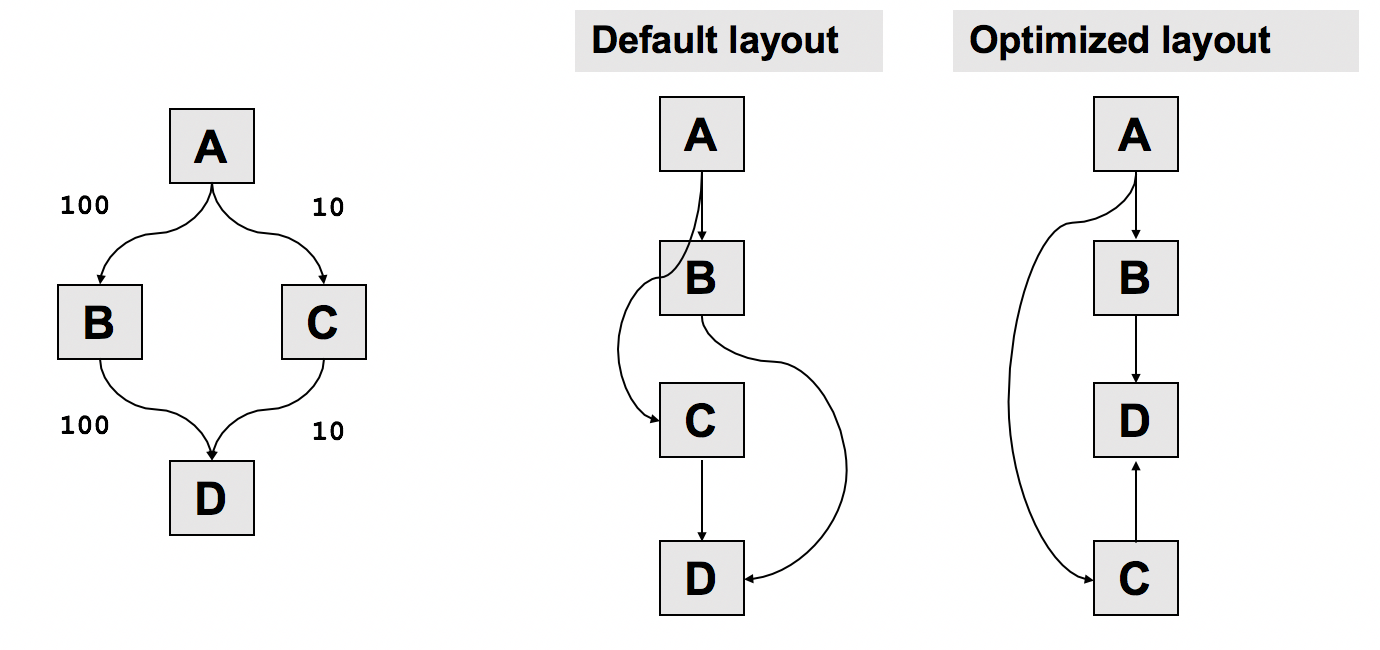
\includegraphics[width=0.6\textwidth]{images/blocklayout.png}
\end{center}

According to the author, the ``dead'' code goes in its own special block. I don't think they actually mean truly dead code, the kind that is compile-time determined to be unreachable, but instead they mean code that never gets invoked in any of the training runs.

So, to sum up, the training data is used to identify what branches are likely to be taken, inlines code where that is a performance increase, and tries to pack the binary code in such a way as to reduce cache misses/page faults. How well does it work?

\subsection*{Benchmark Results}

This table, condensed from~\cite{pogo2} summarizes the gains to be made. The application under test is a standard benchmark suite (Spec2K) (admittedly, C rather than Rust, but the goal is to see if the principle of POGO works and not just a specific implementation):

\begin{center}
\begin{tabular}{l|l|l|l|l|l}
	\textbf{Spec2k:} & \textbf{sjeng} & \textbf{gobmk} & \textbf{perl} & \textbf{povray} & \textbf{gcc}\\ \hline
	\textbf{App Size:} &  {Small} & {Medium} & {Medium} & {Medium} & {Large} \\ \hline
	\textbf{Inlined Edge Count} & 50\% & 53\% & 25\% & 79\% & 65\% \\ \hline
	\textbf{Page Locality} & 97\% & 75\% & 85\% & 98\% & 80\% \\ \hline
	\textbf{Speed Gain} & 8.5\% & 6.6\% & 14.9\% & 36.9\% & 7.9\% \\ 
\end{tabular}
\end{center}

There are more details in the source as to how many functions are used in a typical run and how many things were inlined and so on. But we get enough of an idea from the last row of how much we are speeding up the program, plus some information about why. We can speculate about how well the results in a synthetic benchmark translate to real-world application performance, but at least from this view it does seem to be a net gain.



\bibliographystyle{alphaurl}
\bibliography{459}


\end{document}
